% TODO REVISAR
\subsubsection{Modelo gráfico}
Como se puede observar en la figura \ref{fig:Teacup_sd} el modelo cuenta con 1 (un) stock para modelar la temperatura de la taza, que llamamos \textit{Teacup Temperature}, 2 (dos) auxiliares, que en este caso son constantes, pero podrían ser funciones, una para la temperatura del cuarto, (\textit{Room Temperature}, y otra para el tiempo característico, \textit{Characteristic Time}), y un flujo de salida (outflow) para la perdida de calor de la taza hacia el cuarto,\textit{Heat Loss to Room}, con origen el stock \textit{Teacup Temperature} y destino vacío. 

Las flechas negras indican que el flujo de salida proveniente de \textit{Teacup Temperature} utiliza dicha constantes auxiliares en su función interna para determinar el valor de dicho flujo de salida en cada instante en el tiempo. La flecha azul, indica que dicha función también utiliza el valor del stock \textit{Teacup Temperature} para hacer este cálculo. 

\begin{figure}[!h]
\centering
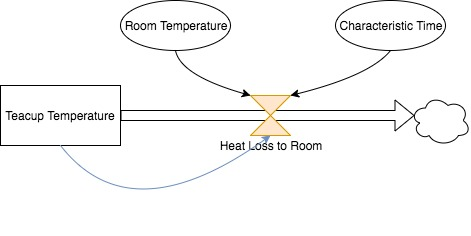
\includegraphics[scale=0.5]{imagenes/Teacup_sd.jpg}
\caption{Modelo Teacup expresado en System Dynamics en formato gráfico}
\label{fig:Teacup_sd}
\end{figure}

\begin{figure}[!h]
\centering
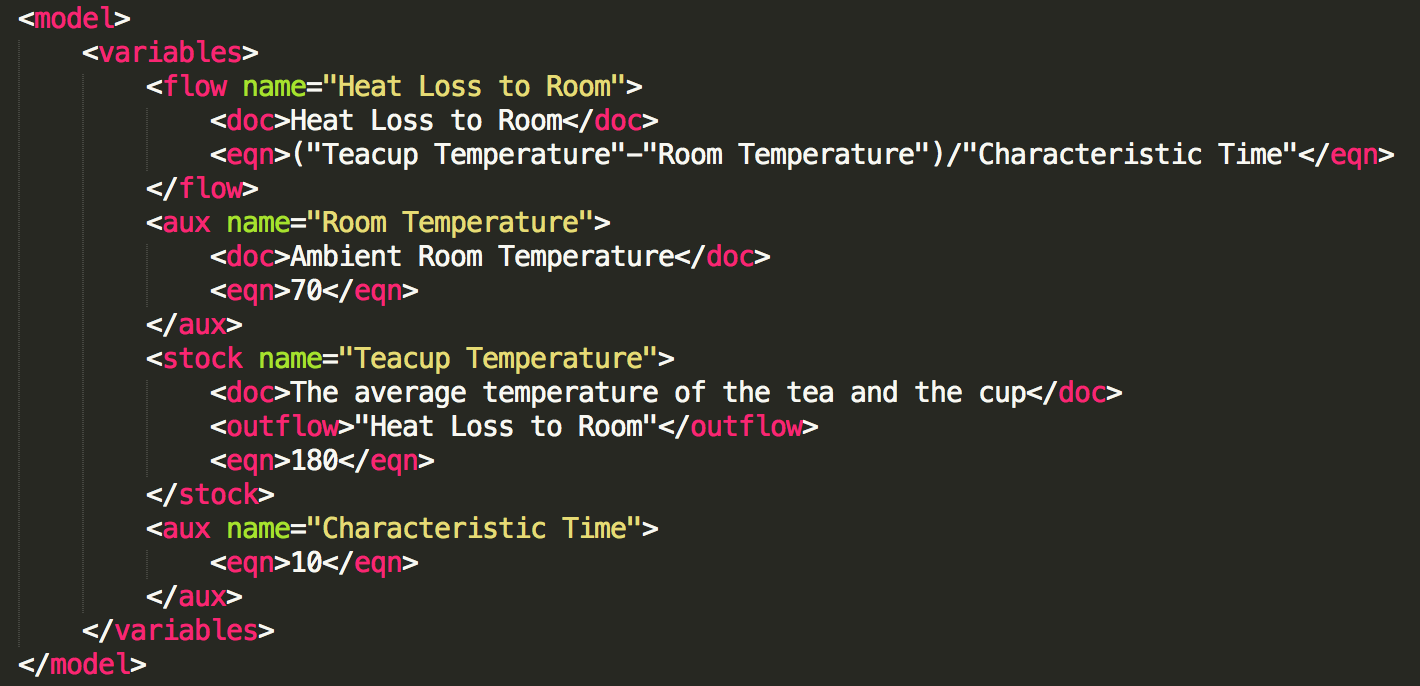
\includegraphics[scale=0.5]{imagenes/teacup_mapeo/Teacup_variables}
\caption{Modelo Teacup exprsado en System Dynamics en formato XMILE}
\label{fig:Teacup_xmile}
\end{figure}

Como se puede observar en la figura \ref{fig:Teacup_xmile}, se utilizan distintos tags para los elementos de System Dynamics, uno para los flujos de output e inflow (el tag \textbf{flow} en el archivo xmile), otro para las constantes auxiliares (el tag \textbf{aux}) y otro para los stocks (el tag \textbf{stock}). 

Asimismo, en cada flujo, se utiliza un tag \textbf{eqn} en archivo xmile para mostrar la función utilizada por dicho \textit{flow} (que puede ser tanto de input ó output) para agregarle o quitarle unidades respectivamente al stock sobre el que operan. 

Observamos que en los stocks y variables auxiliares se utiliza el tag \textbf{eqn} para mostrar el valor inicial de dicho stock ó variable auxiliar. En este caso, las variables auxiliares son todas constantes, con lo cuál en el tag \textbf{eqn} contiene el valor que se mantendrá igual durante toda la simulación.

A partir de estas observaciones, decidimos representar este mismo modelo en el formalismo DEVS, de la forma en que se muestra en el diagrama de la figura \ref{fig:Teacup_devs_flattened}

\begin{figure}[!h]
\centering
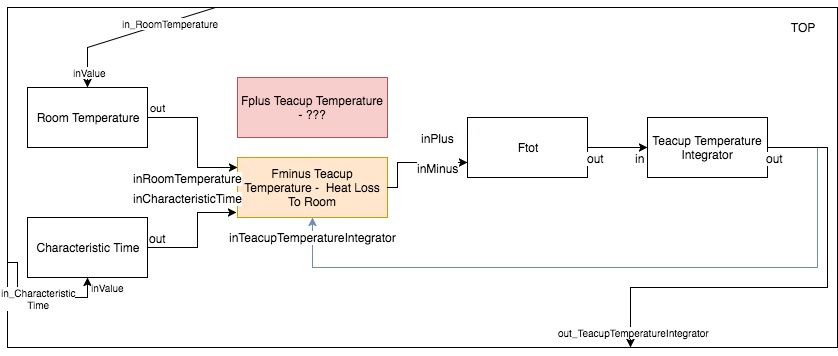
\includegraphics[scale=0.5]{imagenes/Teacup_devs_flattened}
\caption{Modelo Teacup expresado en DEVS en formato gráfico}
\label{fig:Teacup_devs_flattened}
\end{figure}

En el diagrama de la figura \ref{fig:Teacup_devs_flattened} se puede observar lo siguiente: el \textbf{stock} se corresponde en el modelo DEVS con dos atómicos.

\begin{itemize}
	\item Un integrador QSS1 de nombre \textit{"Teacup Temperature Integrator"} (\texttt{utilizamo el nombre del stock más la palabra Integrator})
	\item Un atómico Ftot que determina la variación de unidades que tendrá dicho stock, utilizando todos los inflows y outflows que operan sobre dicho stock ($\sum inflows - \sum outflows $). Los inflows se conectarán al puerto \texttt{inPlus} y los outflows al \texttt{inMinus}. 
\end{itemize}

Por otro lado, a cada flujo (en este caso \textit{Heat Loss to Room} se corresponde con dos atómicos, uno representando el flujo de entrada (\textbf{inflow}) y otro la flujo de salida (\textbf{outflow}). Esto es para darle mejor legibilidad al modelo.

Decidimos nombrarlo de esta manera, en el caso de un \textbf{outflow} concatenando \textit{Fminus} el nombre del \textbf{stock} sobre el cual opera y el nombre del flujo, en el caso del demolo teacup \textit{Fminus Teacup Temperature Heat Loss to Room}.

En el caso de un inflow, el nombre es igual salvo que reemplazamos \textit{Fminus} por \textit{Fplus}. En el ejemplo de la figura \ref{fig:Teacup_devs_flattened}, el atómico que representa el \textbf{inflow} \textit{Heat Loss to Room} de no cumple ninguna función en el modelo DEVS y es por ello que lo marcamos en rojo. 

Finalmente, a los auxiliares (tag \textbf{aux}) del modelo SD se corresponde con atómicos en el modelo DEVS. En este caso, los atómicos emitirán un valor constante a través de su puerto out. Dado que los valores de los auxiliares \textit{Room Temperature} y \textit{Characteristic Time} es utilizado por el flujo \textit{Heat Loss to Room} para el calculo del valor de la función en el modelo SD. En el modelo DEVS estos atómicos se conectarán con los correspondientes a los atómicos del flujo (no realizamos las conexiones al atómico correspondiente al \textbf{inflow} ya que no es utilizado en el modelo).

También podemos observar en el diagrama del modelo DEVS una línea azul la cual se corresponde con la línea azul del diagrama \ref{fig:Teacup_sd} (en el modelo SD esto es la utilización de \textit{Teacup Temperature} en el calculo de \textit{Heat Loss to Room}). De esta forma, mostramos que el atómico \textit{FminusTeacupTemperature - Heat Loss to Room} utiliza también el output del atómico \textit{Teacup Temperature Integrator} para realizar sus cálculos. 

\subsubsection{Múltiples flujos afectando un stock}
Una pregunta que nos hicimos fue, ¿qué pasaría en el caso de que más de un \textbf{outflow} operara sobre \textit{Teacup Temperature}?
Decidimos pensar cómo sería la traducción gráfica del siguiente modelo (figura \ref{fig:Teacup_sd_2}). El mismo tiene un segundo o\textbf{outflow} que opera sobre el \textbf{stock} \textit{Teacup Temperature}, es decir bajando la temperatura de la taza de té, que representa una máquina de enfriamiento (\textit{Cooling Machine} en la literatura), como puede ser por ejemplo un ventilador. El modelo DEVS correspondiente resolvimos debería ser el de la figura \ref{fig:Teacup_devs_flattened_2}. 

Es decir, que se agregan dos atómicos, uno correspondiente al flujo como \textbf{inflow} y otro como \textbf{outflow}, como en el caso de la temperatura perdido en el ambiente (flow \textit{Heat Loss to Room}) sólo el \textbf{outflow} tiene conexiones. El atómico \textit{Ftot} ahora tiene un puerto adicional en uso, para la recepción de los valores \textit{FminsuTeacupTemperature - Heat Loss to Room} como parte de los \textbf{outflows} que operan sobre el \textbf{stock}, recordemos que este atómicos calcula $\sum inflows - \sum outflows $.

\begin{figure}[!h]
\centering
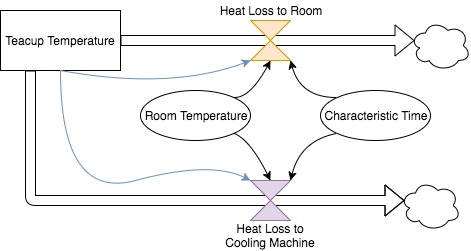
\includegraphics[scale=0.4]{imagenes/Teacup_sd_2}
\caption{Modelo Teacup (versión 2) expresado en SD en formato gráfico}
\label{fig:Teacup_sd_2}
\end{figure}

\begin{figure}[!h]
\centering
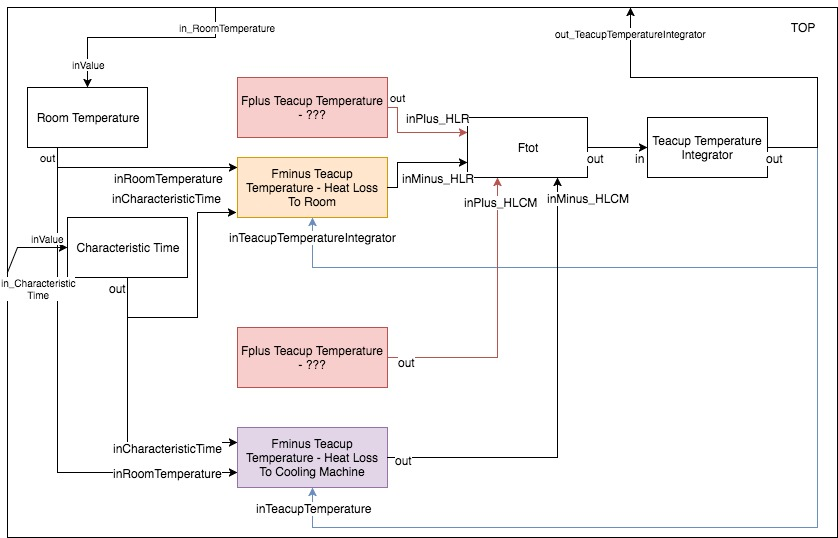
\includegraphics[scale=0.4]{imagenes/Teacup_devs_flattened_2}
\caption{Modelo Teacup (versión 2) expresado en DEVS en formato gráfico}
\label{fig:Teacup_devs_flattened_2}
\end{figure}

\pagebreak

\subsubsection{El modelo en CD++}
Habiendo generado nuestro modelo DEVS para \textit{Teacup} quisimos ver como sería el mismo en \texttt{CD++}, es decir el archivo .ma, así como también las clases  \texttt{C++} que representan a los atómicos. Ya que estos son los archivos que queremos generar una vez traducido el archivo \textbf{xmile} a \textbf{devsml}.

Por cuestiones de tiempo y para simplificar la implementación, sólo trabajamos con la versión aplanada del modelo. Es decir, no buscaremos generar acoplados alrededor de la dinámica de los \textbf{stocks}. Para ver más detalles de como pensamos dichos acoplados ver sección \ref{sssec:cdm}.

\begin{figure}[!h]
\centering
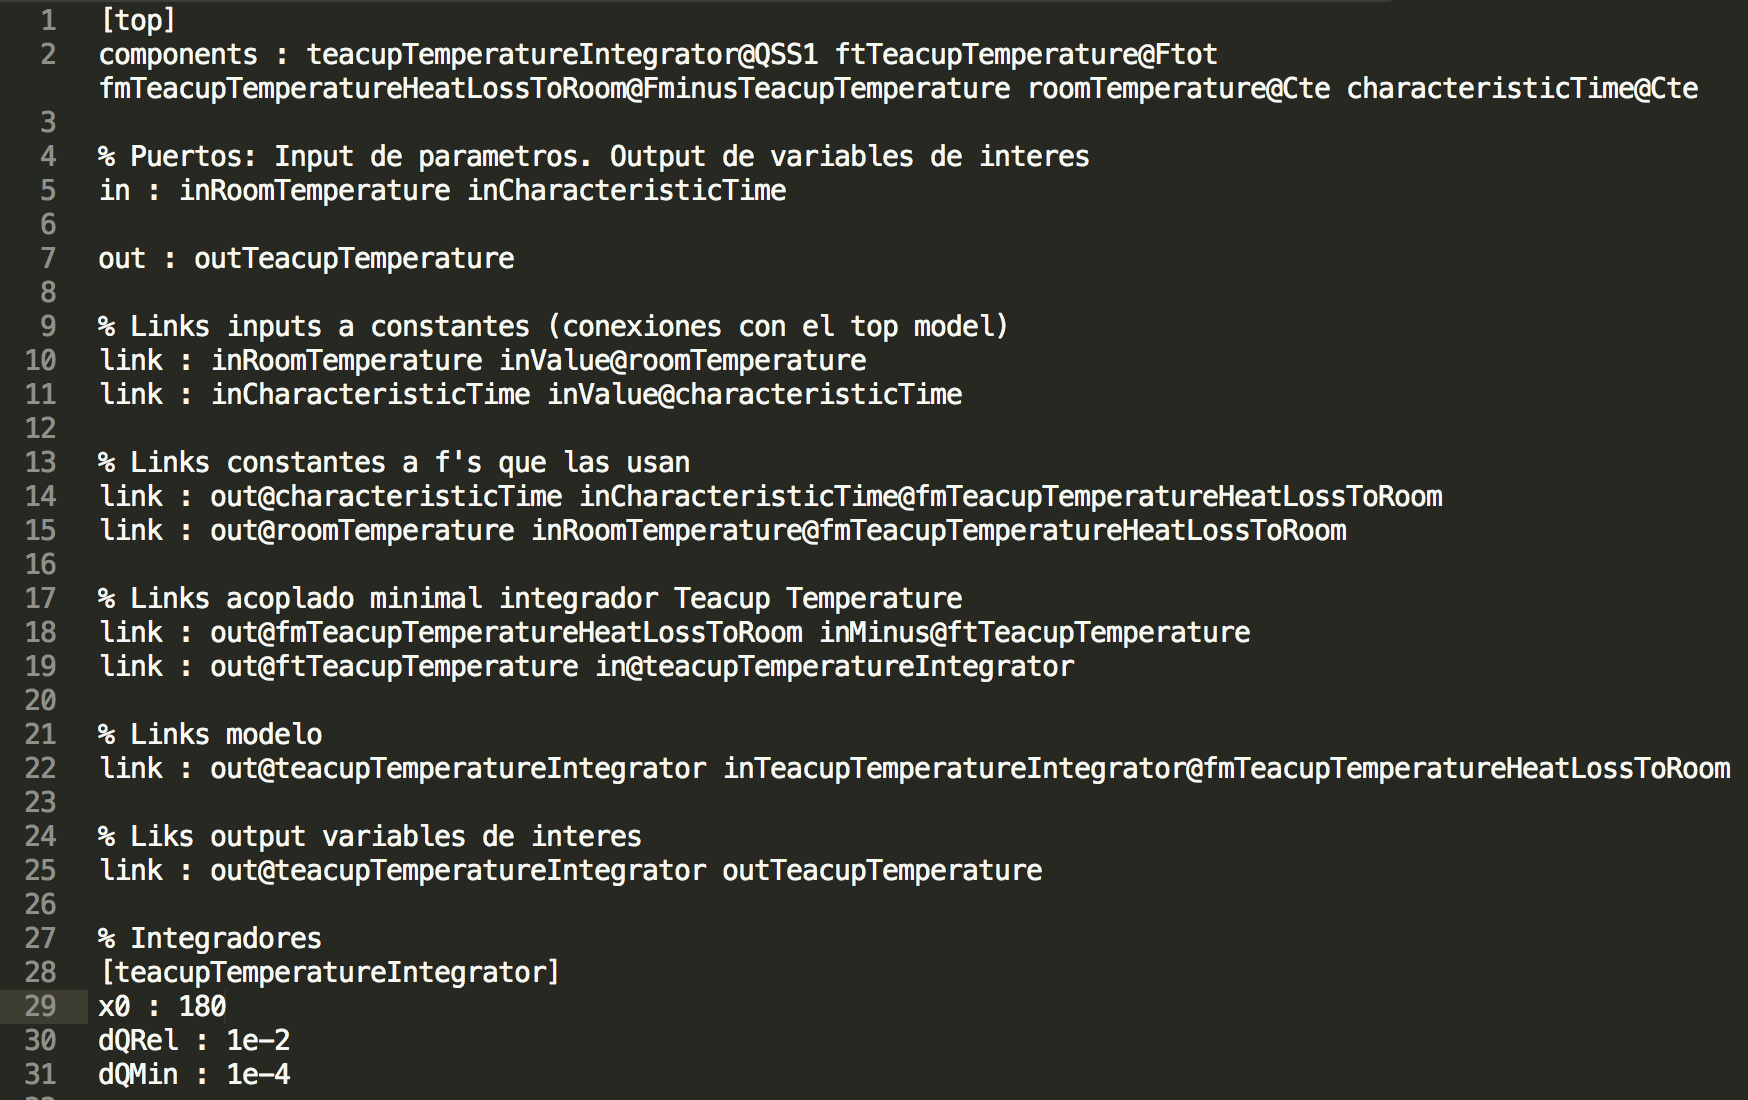
\includegraphics[scale=0.5]{imagenes/teacup_mapeo/Teacup_ma}
\caption{Archivo .ma correspondiente al modelo Teacup para simular el modelo en el simulador CD++}
\label{fig:Teacup_ma}
\end{figure}

Como se puede observar en la figura \ref{fig:Teacup_ma}, el archivo \texttt{.ma} consta de la definición del componente acoplado que engloba todo el modelo (\texttt{[top]}), la definición de todos los componentes que forman parte de este modelo acoplado (en este caso sólo modelos atómicos), los puertos de entrada y salida, así como los links de cada uno de los componentes. En este caso, las entradas son las variables constantes auxiliares y la salida es la única variable de interés del modelo, la temperatura de la taza. 

Si se compara el modelo de la figura \ref{fig:Teacup_devs_flattened} con el archivo \texttt{.ma} de la figura \ref{fig:Teacup_ma}, puede verse una correspondencia entre los descripto en el archivo con el diagrama DEVS.

Ahora bien, los atómicos utilizados en este modelo tienen cierto comportamiento, por tratarse de \texttt{CD++} la implementación será mediante las clases \texttt{C++} que sean necesarias. Por lo que vimos, los atómicos que se necesitan implementar, como \textit{Ftot}, \textit{Fmin} o \textit{Fplus}, tienen un comportamiento similar aunque guardan ciertas diferencias (ej: puertos de entrada, función que computan a la salida,etc.) que podríamos tratar de generalizar para poder generar estas clases de manera automática, generando clases específicas para cada atómico que hiciese falta, o crear clases genéricas que permitan generar las diferencias al momentos de instanciar o inicializar los atómicos. 

Nuevamente por cuestiones simplicidad y tiempo, al momento de realizar la implementación, decidimos ir por la primera estrategia, es decir generamos para cada una de las clases necesarias de los atómicos automáticamente sus correspondientes archivos \texttt{.h} y \texttt{.cpp}.

\begin{figure}[!h]
\centering     %%% not \center
\subfigure[Archvo .h]{\label{fig:Teacup_h}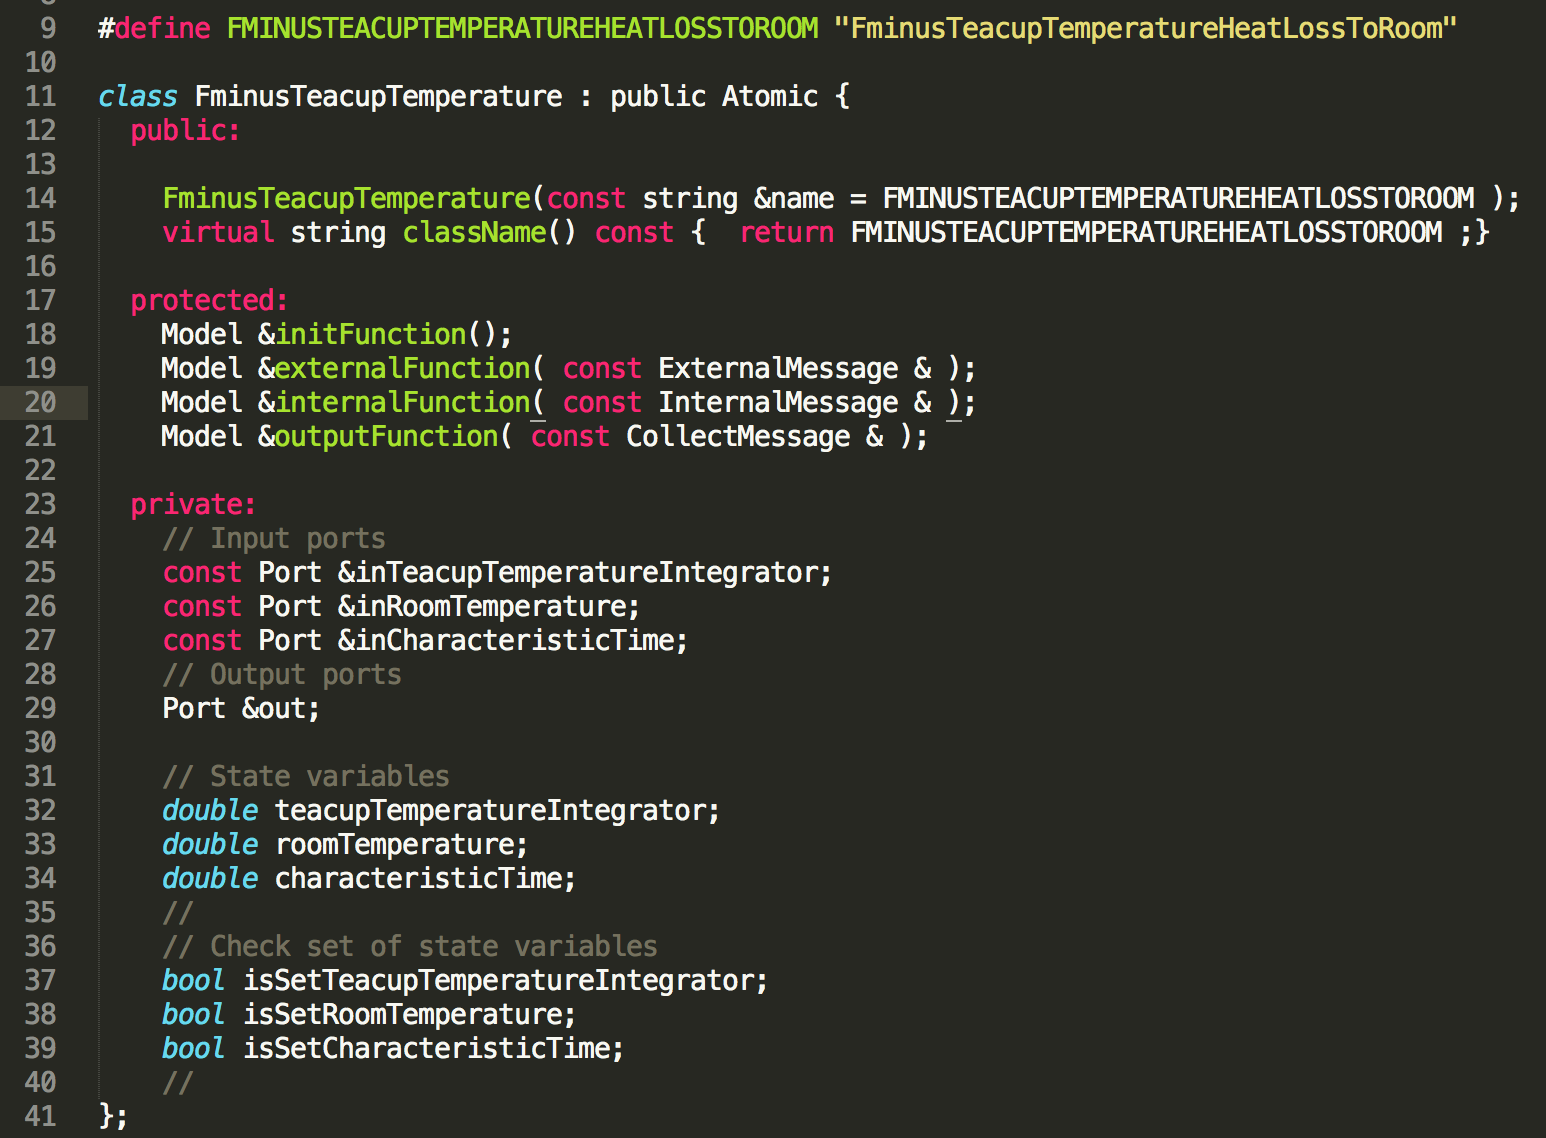
\includegraphics[scale=0.26]{imagenes/teacup_mapeo/Teacup_h}}
\subfigure[Archivo .cpp]{\label{fig:Teacup_hpp}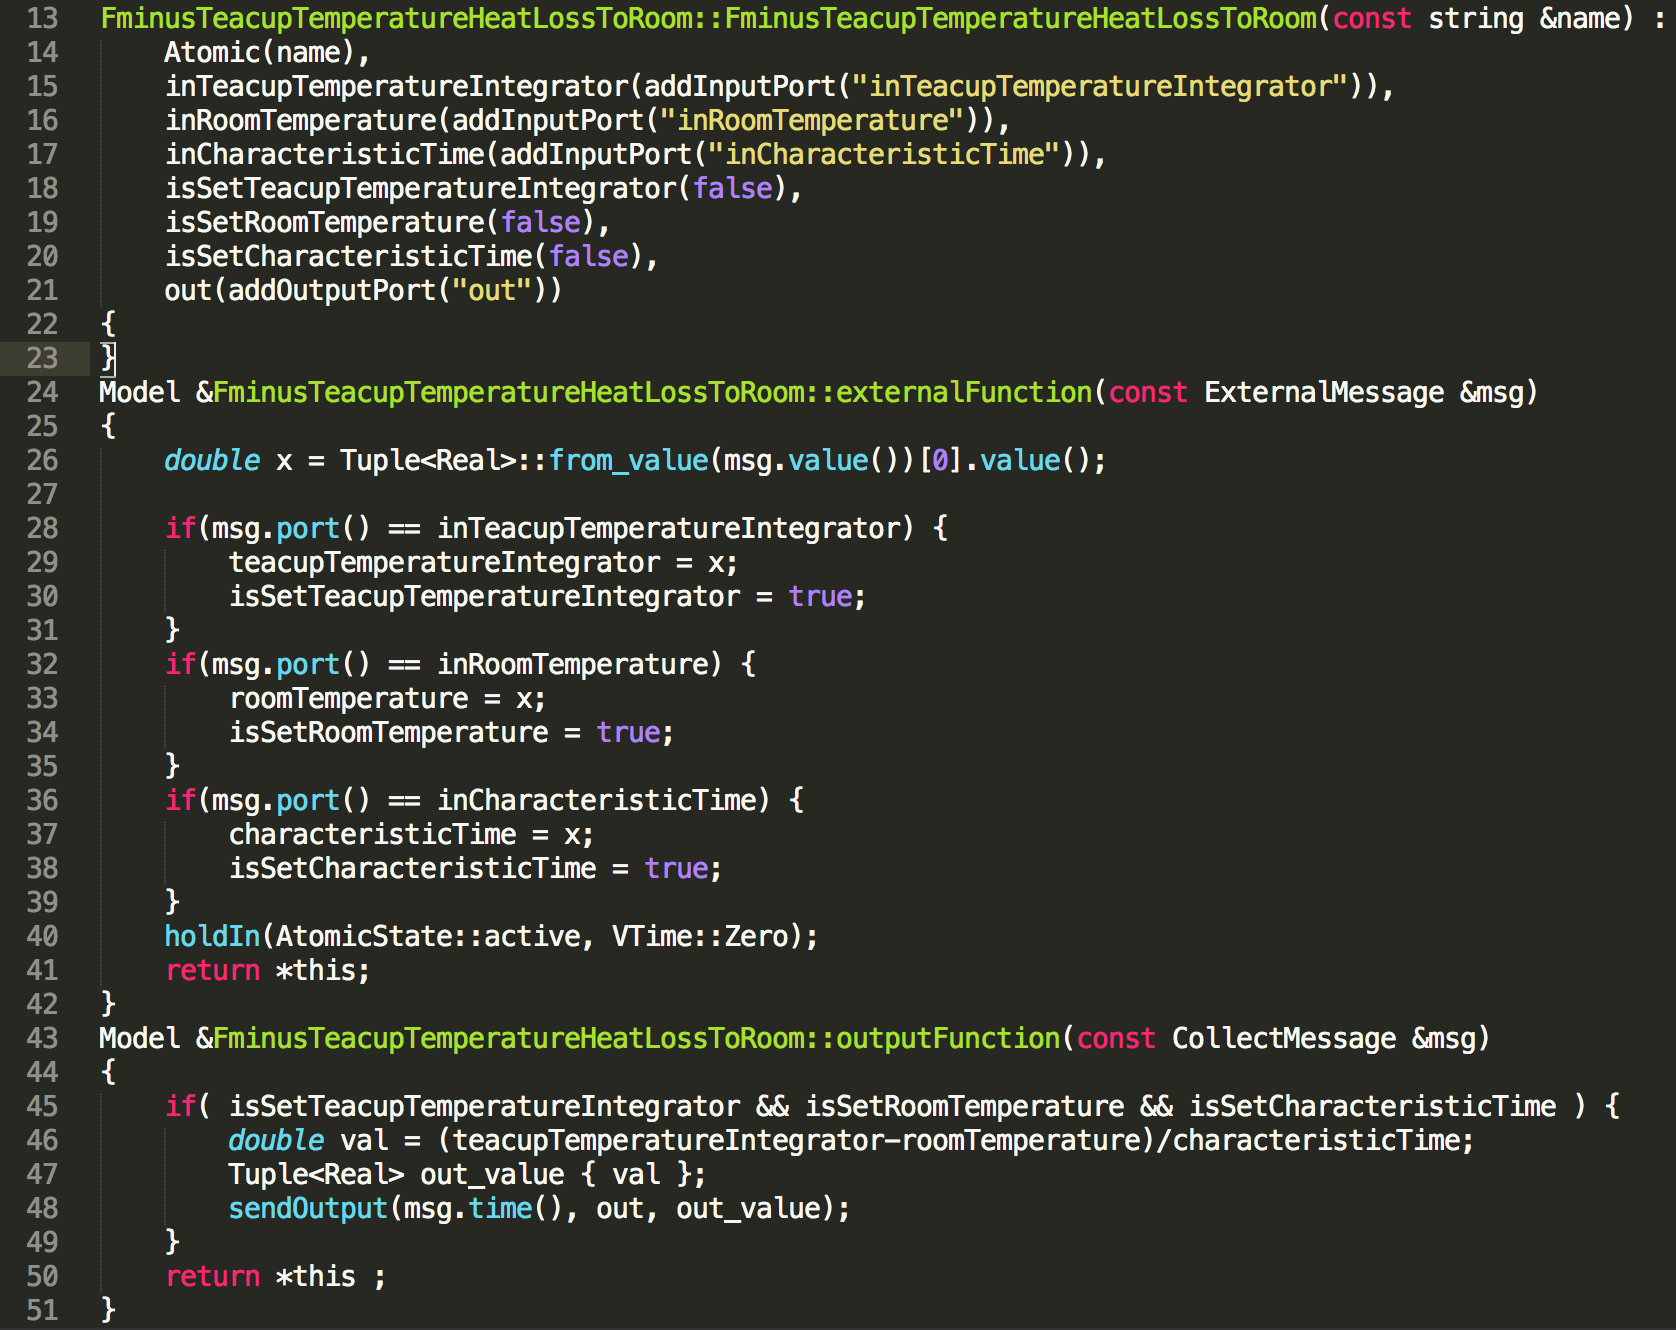
\includegraphics[scale=0.26]{imagenes/teacup_mapeo/Teacup_cpp}}
\caption{Código relevante de los archivos .h y .cpp generados para el atómico FminusTeacupTemperature}
\end{figure}

\begin{figure}[!h]
\centering     %%% not \center
\subfigure[Archvo Ftot.cpp]{\label{fig:Teacup_h}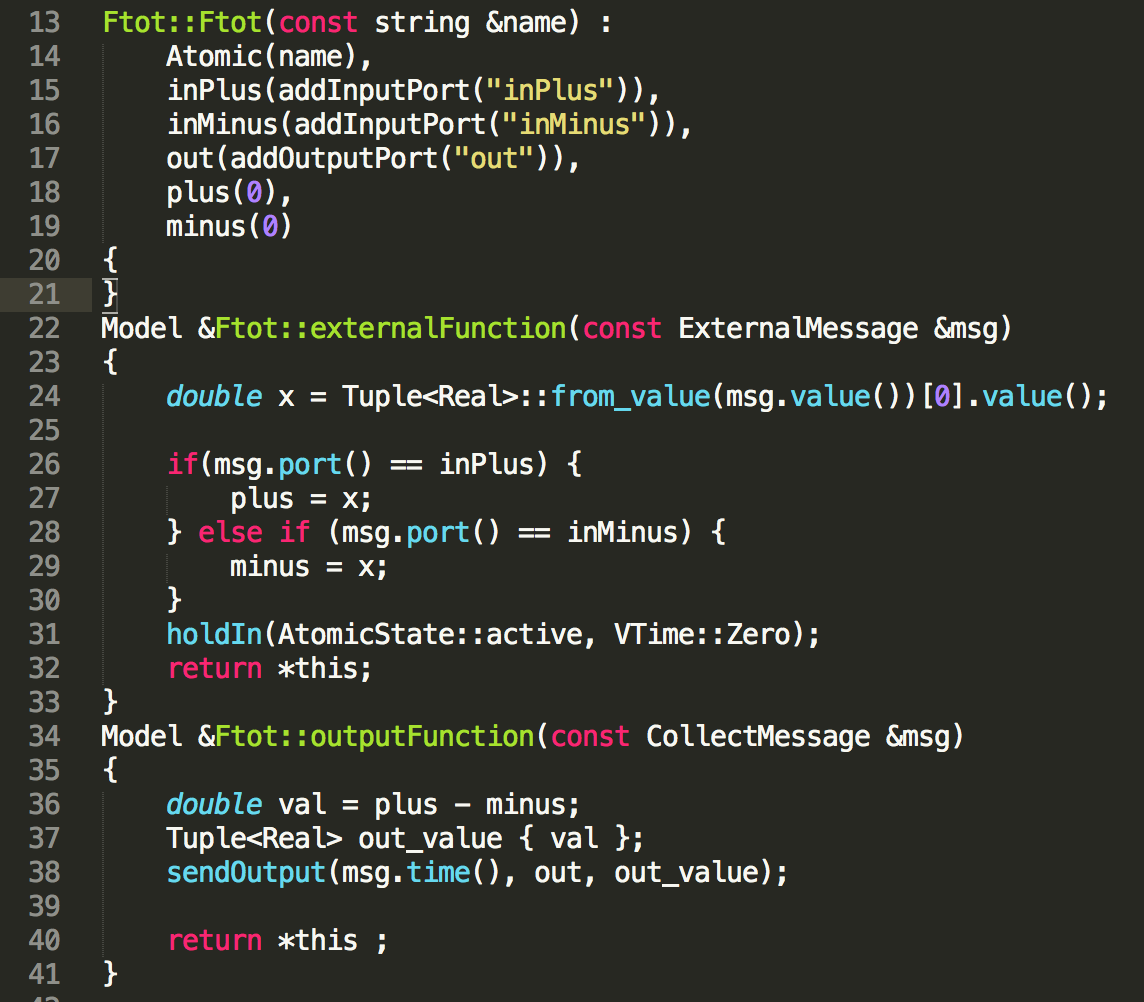
\includegraphics[scale=0.3]{imagenes/gral_mapeo/ftot_cpp}}
\subfigure[Archivo Cte.cpp]{\label{fig:Teacup_hpp}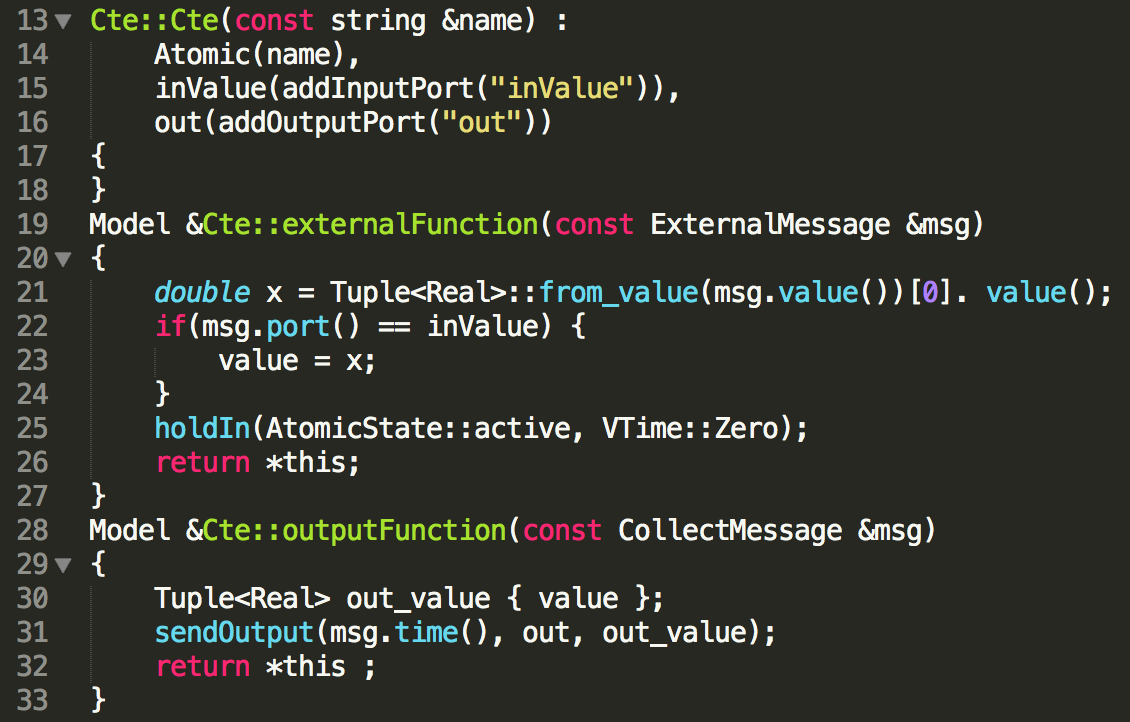
\includegraphics[scale=0.3]{imagenes/gral_mapeo/cte_cpp}}
\caption{Código relevante de los archivos .cpp generados para los atómicos Cte y Ftot}
\end{figure}

\subsubsection{Generación de modelo ejecutable en CD++}
Hemos visto en las secciones anteriores que es posible pasar un modelo en System Dynamics a un modelo DEVS, por lo que sería posible generar a partir de un archivo \texttt{xmile} un archivo \texttt{DEVSML} y a partir de este último generar un archivo \texttt{.ma} y los archivos de necesarios para los atómicos (estos vistos en la sección anterior).

Nos faltaría unicamente revisar el archivo \texttt{DEVSML} del modelo teacup frente al archivo \texttt{.ma} a fin de entender como sería dicha traducción. Como se pueden ver comparando la figura \ref{fig:Teacup_devsml_ports} y \ref{fig:Teacup_devsml_stocks} con la figura \ref{fig:Teacup_ma}, puede verse facilmente la correspondencia de atómicos, puertos y links.

De esta forma, podemos ver que es posible generar las transformaciones necesarias para pasar de un modelo ejecutable especificado en un formalismo de tiempo continuo hacia otro formalismo, de tiempo continuo y eventos discretos.

\begin{figure}[!h]
	\centering     %%% not \center
	\subfigure[Conexiones internas]{\label{fig:Teacup_devsml_internal_connections}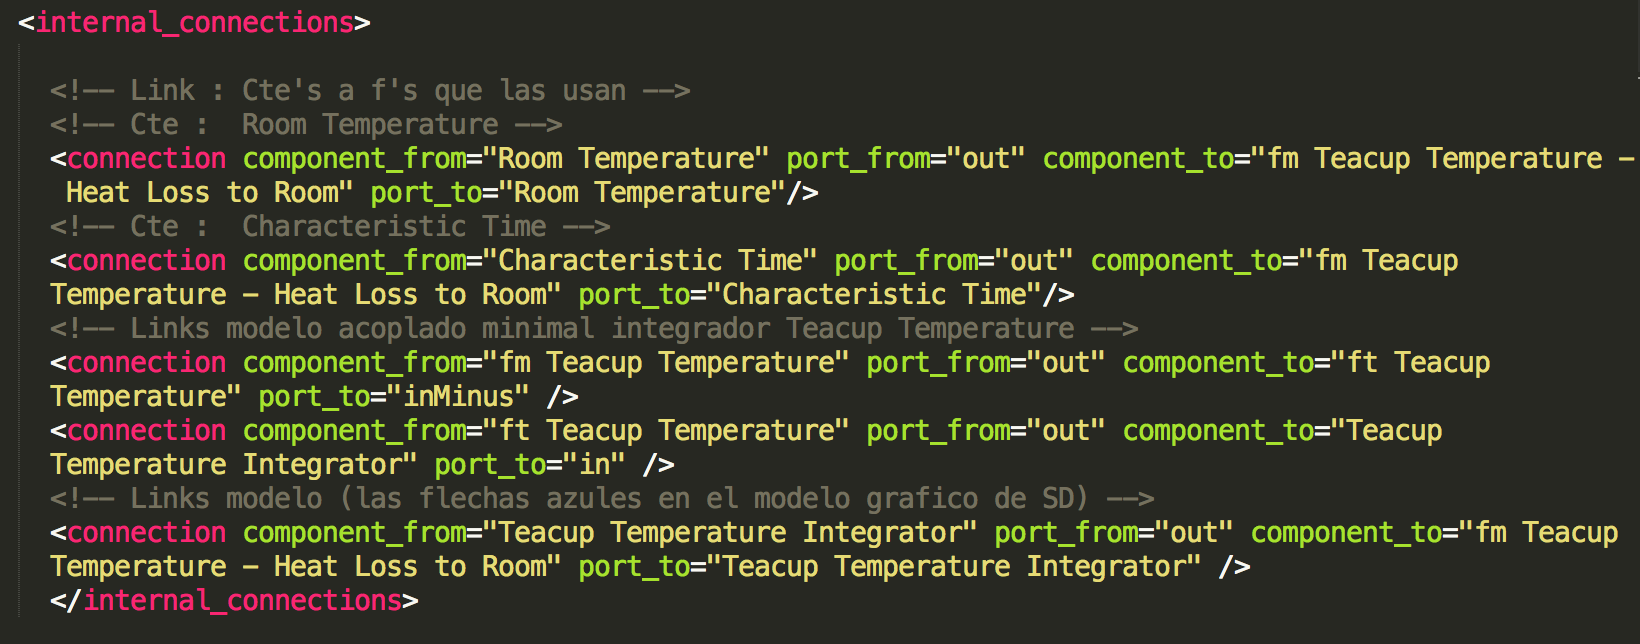
\includegraphics[scale=0.4]{imagenes/teacup_mapeo/Teacup_devsml_internal_connections}}
	\subfigure[Conexiones externas]{\label{fig:Teacup_devsml_external_connections}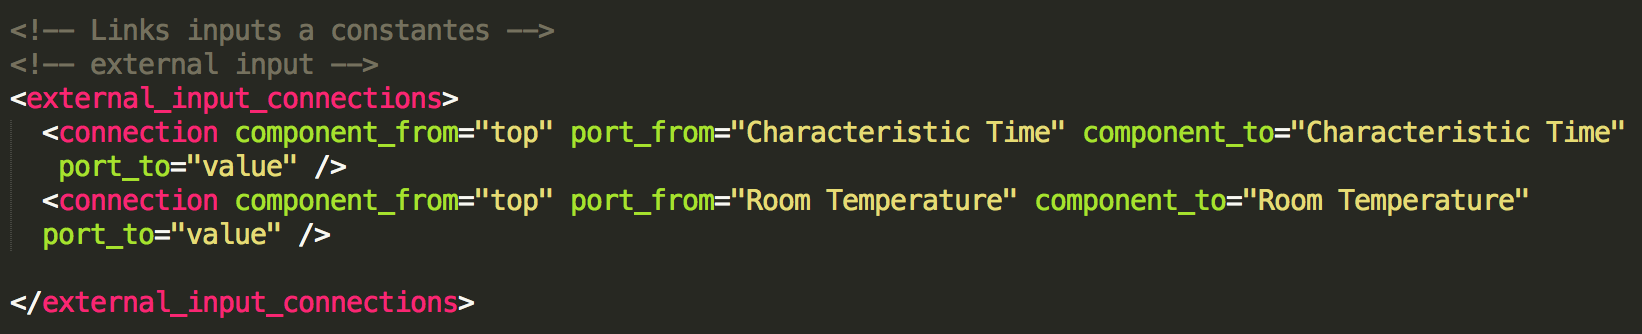
\includegraphics[scale=0.4]{imagenes/teacup_mapeo/Teacup_devsml_external_connections}}
	\subfigure[Puertos de entrada/salida del modelo Top]{\label{fig:Teacup_devsml_ports}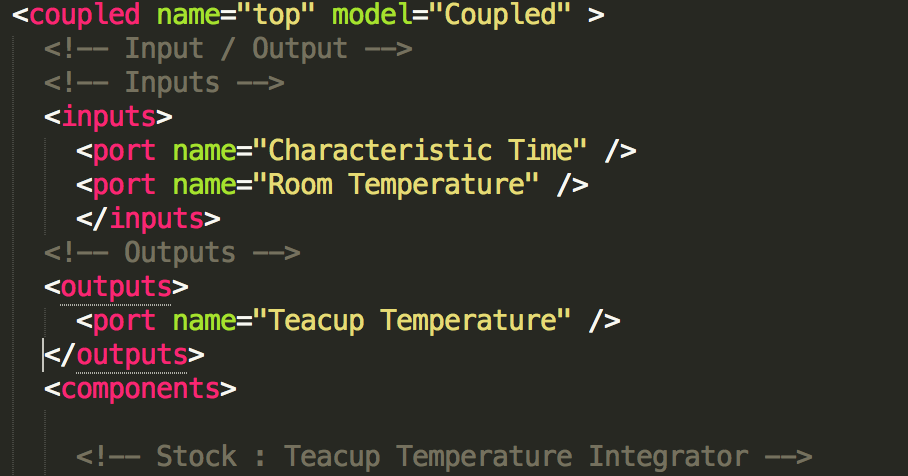
\includegraphics[scale=0.4]{imagenes/teacup_mapeo/Teacup_devsml_ports}}
	\caption{Parte relevante del código .devsml generado por cada conexión y para los puertos del modelo Top}
\end{figure}

\begin{figure}[!h]
\centering     %%% not \center
\subfigure[Atómicos 1-1 para cada Flow]{\label{fig:Teacup_devsml_components}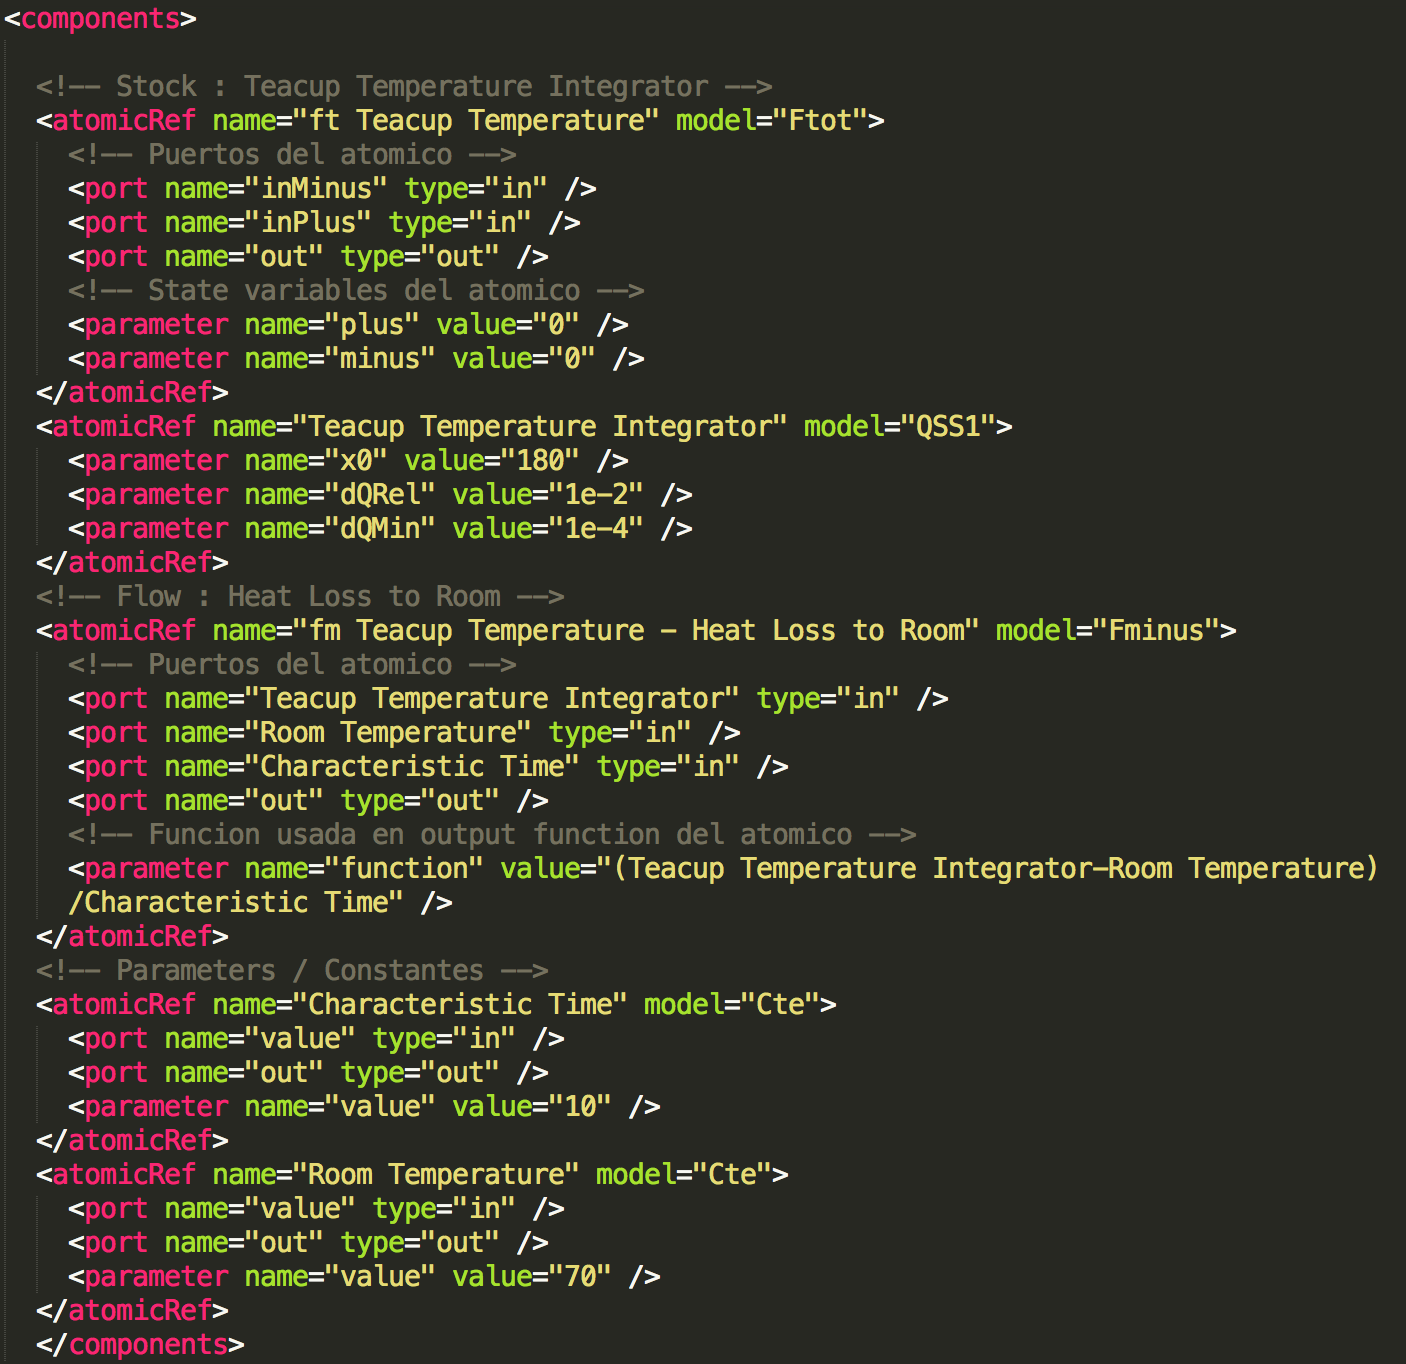
\includegraphics[scale=0.4]{imagenes/teacup_mapeo/Teacup_devsml_components}}
\subfigure[Atómicos 1-1 para cada Stock]{\label{fig:Teacup_devsml_stocks}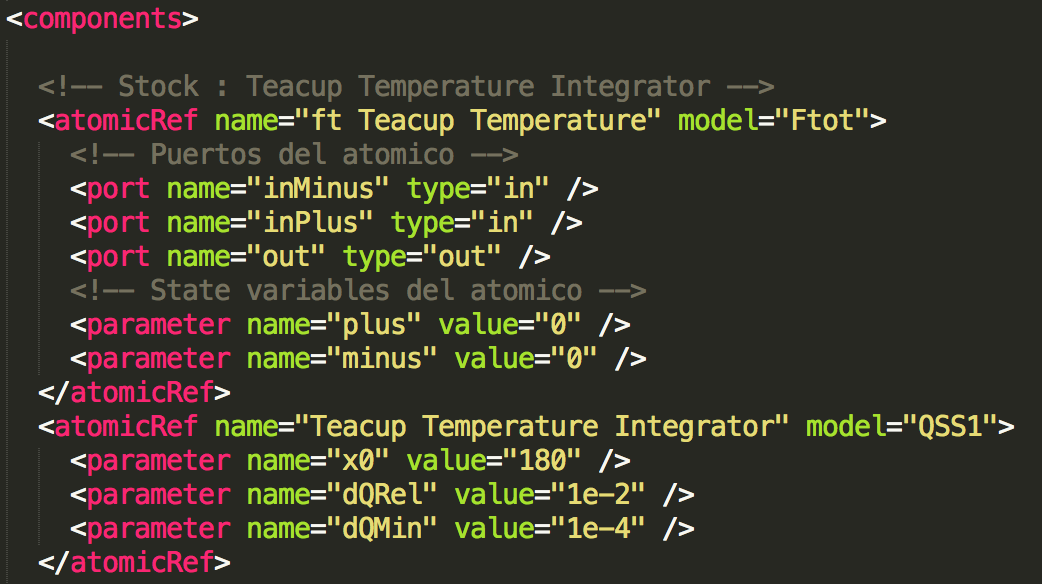
\includegraphics[scale=0.4]{imagenes/teacup_mapeo/Teacup_devsml_stocks}}
\caption{Parte relevante del código .devsml generado por cada Constante, Stock y Flow}
\end{figure}

\pagebreak

\subsubsection{Composibilidad del modelo} \label{sssec:cdm}
¿Es este modelo DEVS obtenido es fácilmente componible con otros? Decidimos ver de que manera era posible modularizar el modelo obtenido, generando un o más acoplados que permitieran componerse con otros.

Si observamos, tanto la temperatura del cuarto como la función características son variables que podrían ser compartidas por otro acoplados de un sistema más complejo, es decir, si una quisiera aislar la dinámica del \textbf{stock} podría pensarlos como variables de entrada. Por lo que dicha dinámica, la del \textbf{stock}, está encapsulada en el atómico integrador y en el \textit{Ftot} y los flujos que lo modifican, en este caso el atómico \textit{Fminus} que representa el flujo de salida (\textbf{outflow}).

Desarrollamos entonces los modelos que se muestra en las figuras \ref{fig:Teacup_devs} y \ref{fig:Teacup_devs_2}, para el modelo original y para la versión con máquina de enfriamiento respectivamente, donde pueden verse los acoplados. 

Todo este análisis nos pareció importante, al momento de desarrollar una primera versión del traductor. Ya que queremos entender de que manera es posible generalizar la forma en que se transformar los modelos SD a modelos DEVS y que además pueda escalar y ser utilizado en modelos más complejos. 

\begin{figure}[!h]
	\centering
	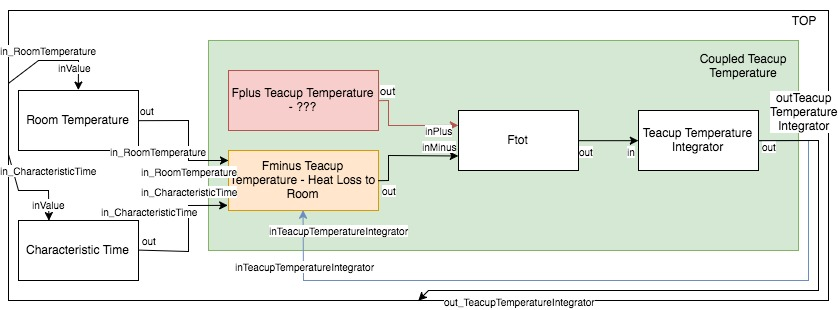
\includegraphics[scale=0.35]{imagenes/Teacup_devs}
	\caption{Modelo Teacup expresado en DEVS en formato gráfico utilizando varios niveles de acoplamiento}
	\label{fig:Teacup_devs}
\end{figure}
\begin{figure}[!h]
	\centering
	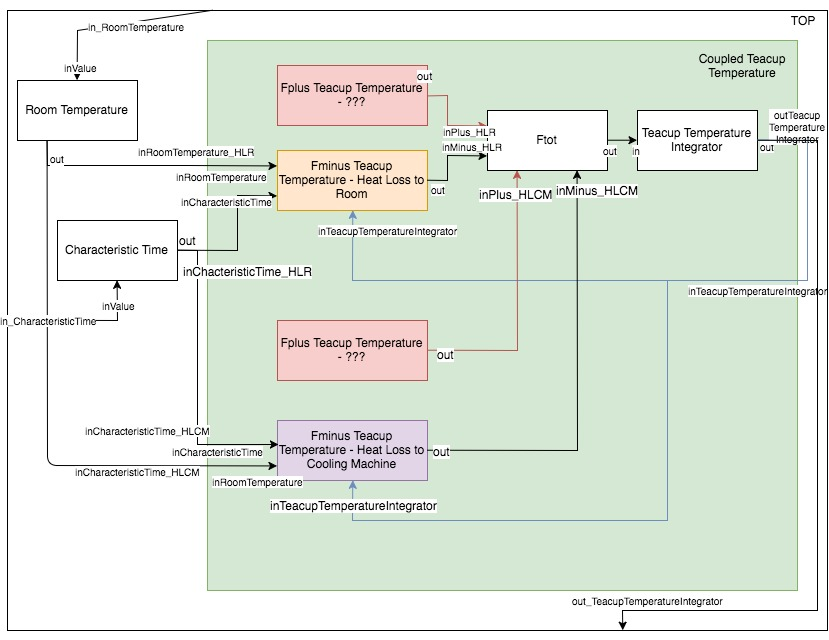
\includegraphics[scale=0.35]{imagenes/Teacup_devs_2}
	\caption{Modelo Teacup (versión 2) expresado en DEVS en formato gráfico utilizando varios niveles de acoplamiento}
	\label{fig:Teacup_devs_2}
\end{figure}
% TODO
\subsection{Modelo Formal}
A modo de completitud mostramos la definición formal de los modelos atómicos 
utilizados en el acoplado Top, con la descripción de su comportamiento interno.
\begin{itemize}

\item \textbf{Cte} : $ roomTemperature, characteristicTime \rightarrow \langle X, S, Y, \delta_{int}, \delta_{ext}, \lambda, t_{a} \rangle$ \newline
\begin{itemize}
	\item $ X = \{ inValue \} $ \newline
	\item $ S = \{ value \} $ \newline
	\item $ Y = \{ out \} $ \newline
	\item $ \delta_{int}(\langle value \rangle) = \emptyset $ \newline
	\item $ \delta_{ext} (\langle value \rangle, e, x)= \{ value := x.value \} $ \newline
	\item $ \lambda(\langle value \rangle, out) = value $ \newline
	\item $ t_{a}(s) = \infty $ 
\end{itemize}

\item \textbf{Fminus} : $ fmTeacupTemperatureHeatLossToRoom \rightarrow \langle X, S, Y, \delta_{int}, \delta_{ext}, \lambda, t_{a} \rangle$ \newline
\begin{itemize}
	\item $ X = \{ inRoomTemperature, inCharacteristicTime, inTeacupTemperatureIntegrator \} $ \newline
	\item $ S = \{ roomTemperature, characteristicTime, teacupTemperatureIntegrator, isSetRoomTemperature, \newline isSetCharacteristicTime, isSetTeacupTemperatureIntegrator \} $ \newline
	\item $ Y = \{ out \} $ \newline
	\item $ \delta_{int}(s) = \emptyset $ \newline
	\item $ \delta_{ext}(s, e, x) = \{
	\\if (x.port = inRoomTemperatureroomTemperature) roomTemperature := x.value; isSetRoomTemperature := true
	\\if (x.port = inCharacteristicTime) characteristicTime := x.value; isSetCharacteristicTime := true
	\\if (x.port = inTeacupTemperatureIntegrator) teacupTemperatureIntegrator = x.value; \\isSetTeacupTemperatureIntegrator := true 
	\} $ \newline
	\item $ \lambda(s, out) = if(todas \ las \ variables \ seteadas) \{ 
\\(teacupTemperatureIntegrator-roomTemperature)/characteristicTime\} \ else \ \emptyset$ \newline
	\item $ t_{a} = \infty $ 
\end{itemize}

\item \textbf{Ftot} : $ ftTeacupTemperature \rightarrow \langle X, S, Y, \delta_{int}, \delta_{ext}, \lambda, t_{a} \rangle$ \newline
\begin{itemize}
	\item $ X = \{ inMinusHeatLossToRoom \} $ \newline
	\item $ S = \{ plus, minus \} $ \newline
	\item $ Y = \{ out \} $ \newline
	\item $ \delta_{int}(\langle plus, minus \rangle) = \emptyset $ \newline
	\item $ \delta_{ext}(\langle plus, minus \rangle, e, x) = \{ 
	\\if (x.port = inPlus) plus := x.value
	\\if (x.port == inMinusHeatLossToRoom) minus := x.value
	\} $ \newline
	\item $ \lambda(\langle plus, minus \rangle, out) = (plus - minus) $ \newline
	\item $ t_{a} = \infty $ 
\end{itemize}
\item \textbf{QSS1} : $ teacupTemperatureIntegrator \rightarrow \langle X, S, Y, \delta_{int}, \delta_{ext}, \lambda, t_{a} \rangle$ \newline
\begin{itemize}
	\item $ X = \{ in \} $ \newline
	\item $ S = \{ ? \} $ \newline
	\item $ Y = \{ out \} $ \newline
	\item $ \delta_{int}(s) = \{ ? \} $ \newline
	\item $ \delta_{ext}(s, e, x) = \{ ? \} $ \newline
	\item $ \lambda(s) = ? $ \newline
	\item $ t_{a} = \{ ? \} $ 
\end{itemize}
\end{itemize}

Ahora que ya tenemos lo atómicos, expresamos el acoplado que utiliza a los atómicos expuestos más arriba:
\begin{itemize}
\item $ Top \rightarrow \langle X, Y, \{ M_{1}, M_{2}, M_{3}, M_{4}, M_{5} \}, C_{xx}, C_{yx}, C_{yy}, Select \rangle$ \newline
\begin{itemize}
	\item $ X = \{ \} $ \newline
	\item $ Y = \{ \} $ \newline
	\item $ M_{1} = roomTemperature $ \newline
	\item $ M_{2} = characteristicTime $ \newline
	\item $ M_{3} = fmTeacupTemperatureHeatLossToRoom$ \newline
	\item $ M_{4} = ftTeacuptTemperature $ \newline
	\item $ M_{5} = teacupTemperatureIntegrator $ \newline
	\item $ C_{xx} = $ \{ \} \newline
	\item $ C_{yx} = \{ (M_{1}.!out, M_{3}.?inRoomTemperture), (M_{2}.!out, M_{3}.?inCharacteristicTime), \\
(M_{5}.!out, M_{3}.?inTecupTemperatureIntegrator), (M_{3}.!out, M_{4}.?inMinusHeatLossToRoom), \\
(M_{4}.!out, M_{5}.?in) \} $ \newline
	\item $ C_{yy} = \{ \} $ \newline
\end{itemize}
\end{itemize}
